\vspace{-0.2cm}
\section{Methods}
\label{sec:methods}
\vspace{-0.1cm}

\begin{figure}[t]%[!htb]
	\centering
	\begin{subfigure}[t]{1\textwidth}
		\centering
		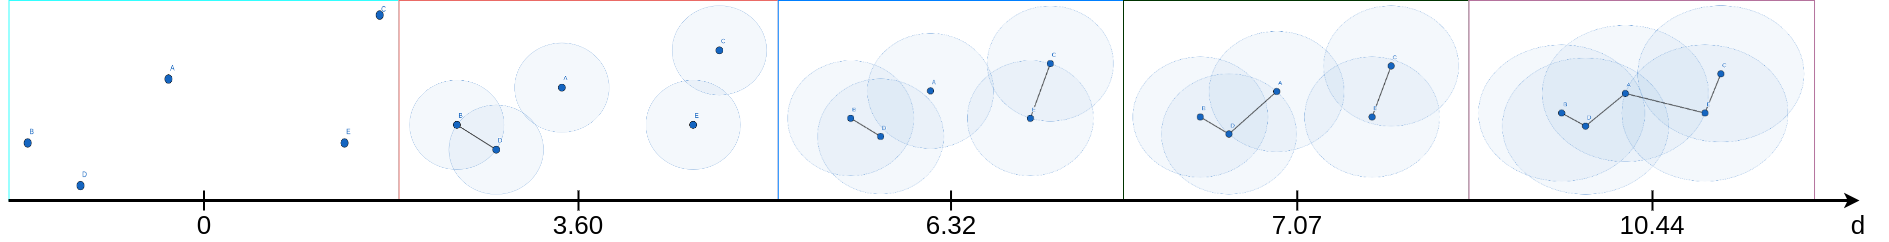
\includegraphics[width=1\textwidth, trim={0cm, 0.0cm, 0.0cm, 0.0cm}]{figures/barcodes_generation_border.png}\hfill
		%\hspace{-15mm}
		\subcaption{Vietoris-Rips filtration on FCN with the parameter $\epsilon$}
	\end{subfigure}
	\hfill
	\begin{subfigure}[t]{1\textwidth}
		\centering
		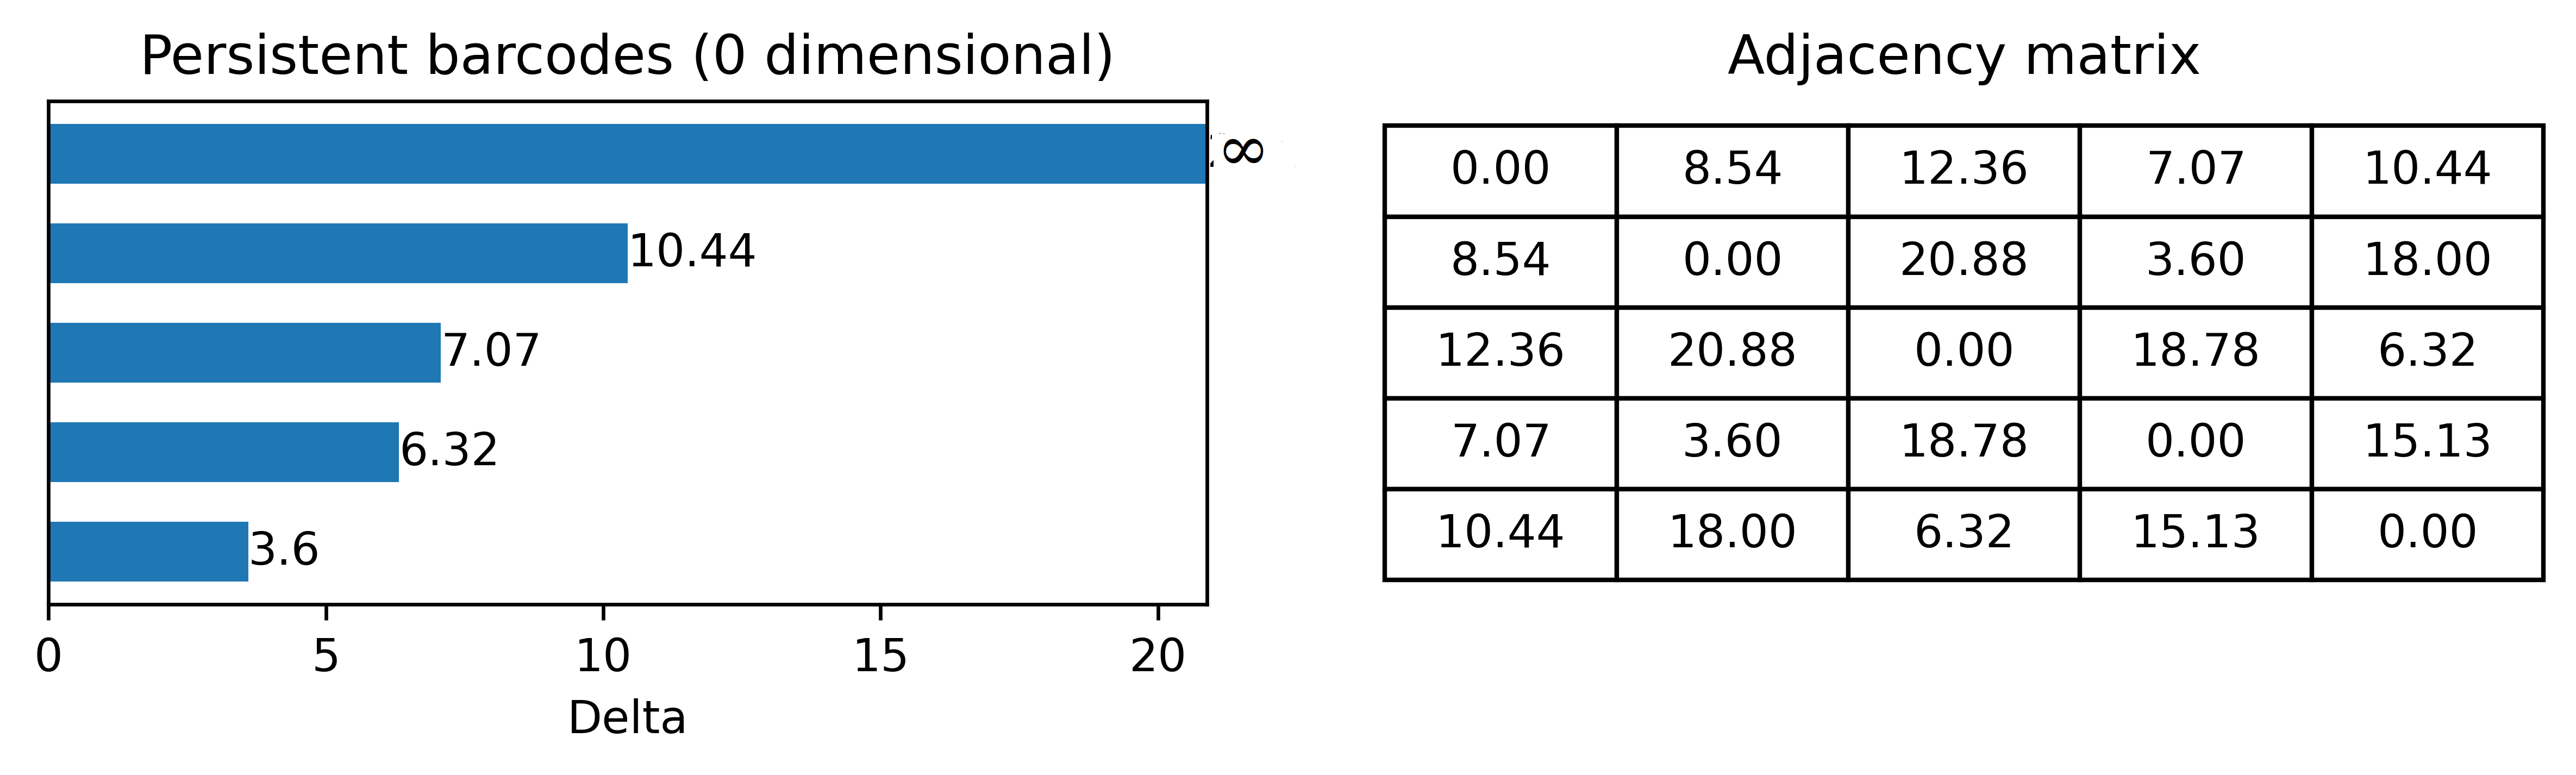
\includegraphics[width=1\textwidth, trim={0cm, 0.0cm, 0.0cm, 0.0cm}]{figures/barcode_matrix_title.png}\hfill
		%\hspace{-15mm}
		\subcaption{0-dimensional persistent barcodes (left) and adjacency matrix of the FCN (right)}
	\end{subfigure}
	\hfill
	\caption{An example of persistent homology to extract topological features using 0-dimensional barcodes. The adjacency matrix is of size $5 \times 5$.}
	\label{fig:rips_new}
\end{figure}
Persistent homology permits analysing a range of thresholds to gather connectivity information from FCN. Figure~\ref{fig:rips_new} shows an example of using persistent homology to record the changes of topological features over the changes of distances using zero-dimensional barcodes. Vietoris-Rips filtration on the given $5 x 5$ FCN is applied to capture the changes in the number of connected components for different parameters of $d$. We use an identical technique to capture topological features from fMRI FCNs extracted using different data acquisition parameters such as three different temporal sampling periods (2500ms, 1400ms, 645ms). We developed TDA based pipeline to illustrate the similarity of the extracted FCNs using the different temporal sampling periods. The TDA pipeline is formed mainly in three steps. First, we create FCNs from rs-fMRI data. Then we extract the persistent barcodes from the FCNs. Finally, we apply statistical analysis to show the similarity between extracted FCNs. This work aims to illustrate the potency of using persistent homology in capturing useful facts from fMRI datasets, proving the PH technique's resiliency towards the data acquisition parameters. To ensure the resiliency of the TDA pipeline, we also developed a nonTDA pipeline using the correlation coefficients of the fMRI datasets. 

Our TDA pipeline has the following steps:

\begin{enumerate}
    \item \textbf{Generate FCNs from rs-fMRI data}: We applied Pearson correlation on the fMRI dataset to generate the FCNs on different data acquisition parameters (2500ms, 1400ms, 645ms) as a data pre-processing step (Section~\ref{sec:fmri_to_fcn}).
    \item \textbf{Create distance matrix from FCNs}: The extracted FCNs are then converted into distance matrices as a weighted graph representing the correlation between time periods (Section~\ref{sec:fcn_to_ms}).
    \item \textbf{Extract persistent barcodes from distance matrix}: In this step, we extract persistent diagrams (0-dimensional barcodes) from the distance matrices using persistent homology to identify the topological features from the correlated matrices (Section~\ref{sec:ms_to_pd}).
    \item \textbf{Statistical analysis on PD to prove the resiliency of different data acquisition parameters}: Finally, we apply statistical analysis on the extracted barcodes to see the similarity between the topological features extracted using different data acquisition parameters (Section~\ref{sec:si}).
\end{enumerate}


\begin{figure}[t]%[!htb]
	\centering	
	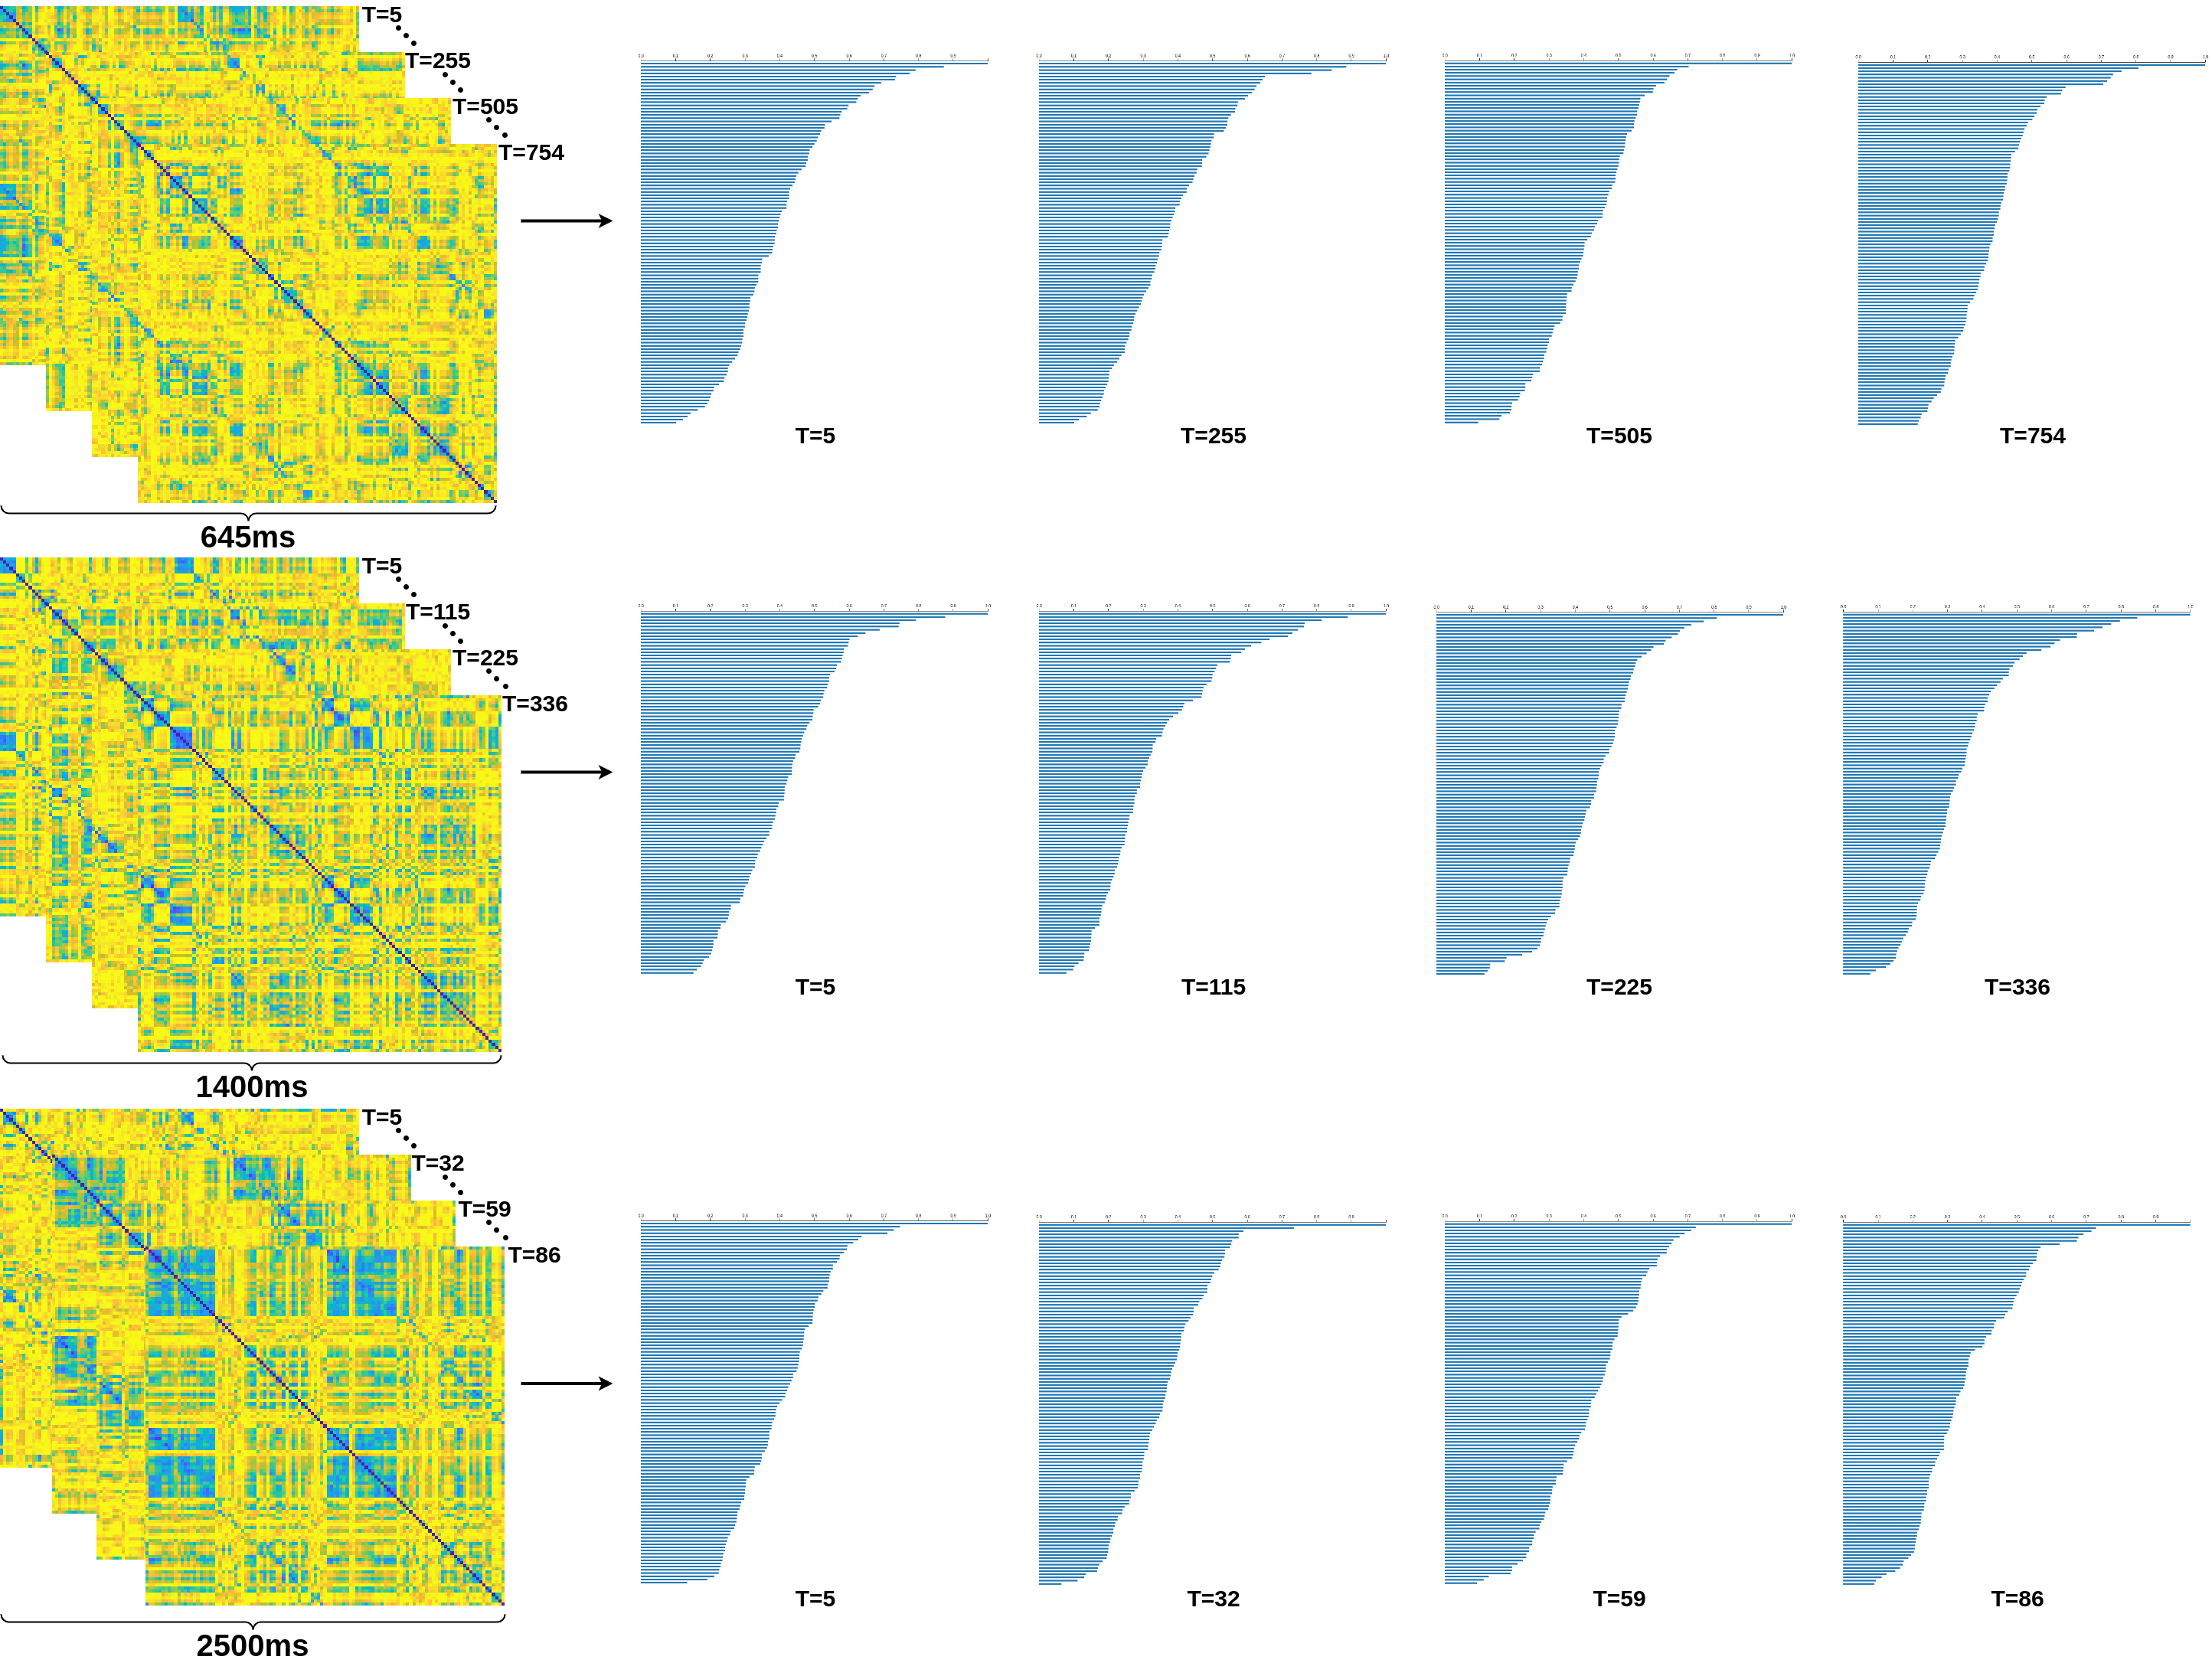
\includegraphics[width=1\textwidth, trim={0cm, 0.0cm, 0.0cm, 0.0cm}]{figures/stacked.png}
	\caption{The FCN and extracted topological feature as 0-dimensional barcodes for subject $32$ at different time points for temporal sampling periods $645ms$ (top), $1400ms$ (center), and $2500ms$ (bottom). The matrix size is $113 \times 113$.}
	\label{fig:wd1}
\end{figure}

\subsection{FCN generation from fMRI data}
\label{sec:fmri_to_fcn}
\textcolor{red}{
Structural T1-weighted and rs-fMRI data were obtained from the openly available Enhanced Nathan Kline Institute Rockland Sample database (NKI-RS)~\cite{nooner2012nki}. 
The MRI data were obtained using a 3T Siemens Magnetom Tim Trio scanner. 
The data acquisition parameters for the T1-weighted structural data were: $1.0$ mm isotropic voxels with 176 slices, 
repetition time (TR) = $1900$ ms,
echo time (TE) = $2.52$ ms and field of view (FOV) = $250 \times 250$.
Resting state fMRI data were acquired using multiband echo-planar imaging (EPI)~\cite{feinberg2010multiplexed} from each subject using three different acquisition protocols with different parameters as follows. 
(1) $3.0$ mm isotropic voxels with $40$ slices, \emph{TR = 645 ms}, TE = $30$ ms, FOV = $222 \times 222$ mm, number of volumes = $900$, andmulti-band factor = $4$.
(2) $2.0$ mm isotropic voxels with $64$ silces, \emph{TR = 1400 ms}, TE = $30$ ms, FOC = $224 \times 224$ mm, number of volumes = $404$ and multi-band factor = $4$. (3)
$2.0$ mm isotropic voxels with 38 slices, \emph{TR = 2500 ms}, TE = $30$ ms; FOV = $216 \times 216$ mm, number of volumes = $120$ and multi-band factor = $1$.
It can be seen that even though we identify the three datasets from each subject with the corresponding TR, the data differ in many other scan parameters such as number of volumes, multiband factor, FOV and voxel size.
}

\textcolor{red}{
The MRI data were subjected to a standard pre-processing pipeline, including the first five volume removal, slice time correction and motion correction. T1-weighted anatomical images were coregistered to the mean functional images, using which the fMRI images were spatially registered to a standard MNI152 template. Nuisance variables such as low-frequency drifts and motion parameters were regressed out. Unwanted physiological fluctuations (white-matter and cerebrospinal fluid signals) were removed using aCOMPCor (anatomical component-based noise correction). After removing subjects that failed quality control, 316 subjects were identified to have usable data from all three acquisition protocols. Subsequently, mean time series from 113 brain regions (obtained using the Yeo parcellation template ~\cite{thomas2011organization}) were obtained for each subject and acquisition protocol.
Using Pearson’s correlation, FCN matrices were estimated from these mean time series. 
}

At this stage, we generate one FCN for each fMRI scan. Each FCN is stored as a symmetric adjacency matrix $M$ with size $113 \times 113$, where $M_{ij}$ represents the correlation coefficient between brain nodes $i$ and $j$. The dataset consists of three temporal frequencies ($645$ms, $1400$ms and $2500$ms). There are $316$ subjects for each temporal frequency. The $2500$ms temporal frequency has 86 timesteps, $1400$ms has 336 timesteps, and $645$ms has 754 timesteps. The total number of adjacency matrices is $371,616$ $(316 \times 86) + (316 \times 336) + (316 \times 754)$ with a dimension of $113 \times 113$. Figure~\ref{fig:wd1} shows an example of the FCN for subject $31$, for the three sampling periods ($645$ms, $1400$ms and $2500$ms).


\subsection{Creation of matrices from FCNs}
\label{sec:fcn_to_ms}

Usually, topological data analysis uses point cloud data in metric configuration. We confine the weighted networks from fMRI data in distance matrices in our TDA pipeline before applying TDA techniques. Then, we extract persistent barcodes from the distance matrices. 


We use popular Pearson’s correlation coefficients $pcc(p_t, q_t)$ to measure the interrelation between any two data points (nodes) $p_t$ and $q_t$ at time $t$ in the fMRI data as it is independent on FCN construction method ~\cite{smith2011network}. This technique ensures that to map of the higher correlations between the data points to a smaller value. The mapping for the distance matrix calculation is:

\[
\mathit{d(p_t, q_t)} = 
\sqrt{ 1 - pcc(p_t, q_t)^2 }
\]

The temporal indexing $t$ indicates this is a temporal dataset, and the correlations and distances are calculated between node pairs at each time point.

\subsection{Extract persistent barcodes from distance matrix}
\label{sec:ms_to_pd}

Using persistent homology, we capture topological features from the distance matrices extracted from the fMRI FCNs. This section overviews topological feature extraction using persistent barcodes and the distance metric we have used. The existing literature contains the details on these topics ~\cite{edelsbrunner2008surveys, Topology_and_data}.

\subsubsection{Extraction of topological features using persistent homology}

Persistent homology can extract topological features from a topological space. The homology of the space can be divided into groups based on the dimensions of the features. A topological space $\mathbb{X}$ can be divided into homology groups $H_i(\mathbb{X})$ for $i={0, 1, 2, ...}$ where $H_i(\mathbb{X})$ represents the $i^th$ homology group. Each homology group $H_n(\mathbb{X})$ denotes the number of n-dimensional holes in the topological space $\mathbb{X}$. For example, the $H_0(\mathbb{X})$ homology group shows the number of connected components, $H_1(\mathbb{X})$ homology group shows the number of holes, $H_2(\mathbb{X})$ homology group shows the number of voids in the topological space $\mathbb{X}$. 

In this paper, we use $H_0(\mathbb{X})$ homology group (0-dimensional) to extract the number of connected components from the rs-fMRI FCNs as topological features. Figure \ref{fig:rips_new} shows a simple example of using persistent homology to extract the topological features from a given FCN. The table at the bottom right in Figure \ref{fig:rips_new}(b) represents the adjacency matrix of an FCN with five nodes. Persistent homology captures the changes in topological features over distance thresholds ($\epsilon$) between the nodes. In a point cloud, $F$ with $p$ nodes, two nodes ($x$, $y$) are marked as connected with an edge if the distance $d(x, y)$ is less than threshold $\epsilon$. In this scenario, they form a 1-Simplex. When three nodes are connected with each other for some value of $\epsilon$, they form 2-Simplex and so on. For a given $\epsilon$, the graph is called a Rips complex represented by $Rips(F , \epsilon)$. These continuous changes in the value of $\epsilon$ result in the changes in topological features. Vietoris-Rips filtration captures the increasing value of $\epsilon$ for which a new Rips-complex, in another word, new topological feature, is being generated \cite{bauer2021ripser}. Figure \ref{fig:rips_new}(a) shows the extraction of different topological features in various thresholds of $\epsilon$ using Vietoris-Rips filtration. 

For each real number $t$ where topological features are changed, we consider them important events and store these values of $t$. For instance, at some time $t_0$, a topological feature, a component is being created, and at time $t_1$, it is merged with another component. We keep track of the $birth$ as $t_{birth} = t_0$ and $death$ as $t_{death} = t_1$ for each component. The time of the $(t_{birth}, t_{death})$ of the topological features is visualized as $barcodes$. The span of time for each feature $t_{death} - t_{birth}$ is called as persistence of that feature. Figure \ref{fig:rips_new}(b)(left) shows the barcodes for the given FCN. At $t=0$, five topological features are born as five independent (connected) components. At $t=3.6$, two components are merged; thus, the death of a component is recorded at $t=3.6$. Therefore, the persistence of that component is $3.6$. Similarly, at $t=6.32$, another component is merged with a persistence of $6.32$. For 0-dimensional persistence barcodes, this process continues until there is only one connected component. This last component never dies; thus, the persistence of this component is $\infty$. The 0-dimensional persistence barcodes in Figure \ref{fig:rips_new}(b)(left) represent the $birth$ and $death$ of the topological features, which is the changes in the number of connected components of the FCN. Each horizontal bar begins at the birth of a component and ends at the death of each component in the barcodes representation. 

In our pipeline, we generate 0-dimensional persistent barcodes for each FCN. Each FCN has $113$ vertices that form the finite set of points $F$ where the value $d_i$ represents the pairwise distance between the points. We extract 0-dimensional barcodes using persistent homology for all the $371,616$ FCNs $((316 \times 86) + (316 \times 336) + (316 \times 754))$. An illustration of the extracted barcodes at $timestep=1$ for all three temporal sampling periods ($645ms$, $1400ms$, $2500ms$) for a single subject is shown in Figure \ref{fig:wd1}.


\begin{figure}[!ht]
	\centering	
	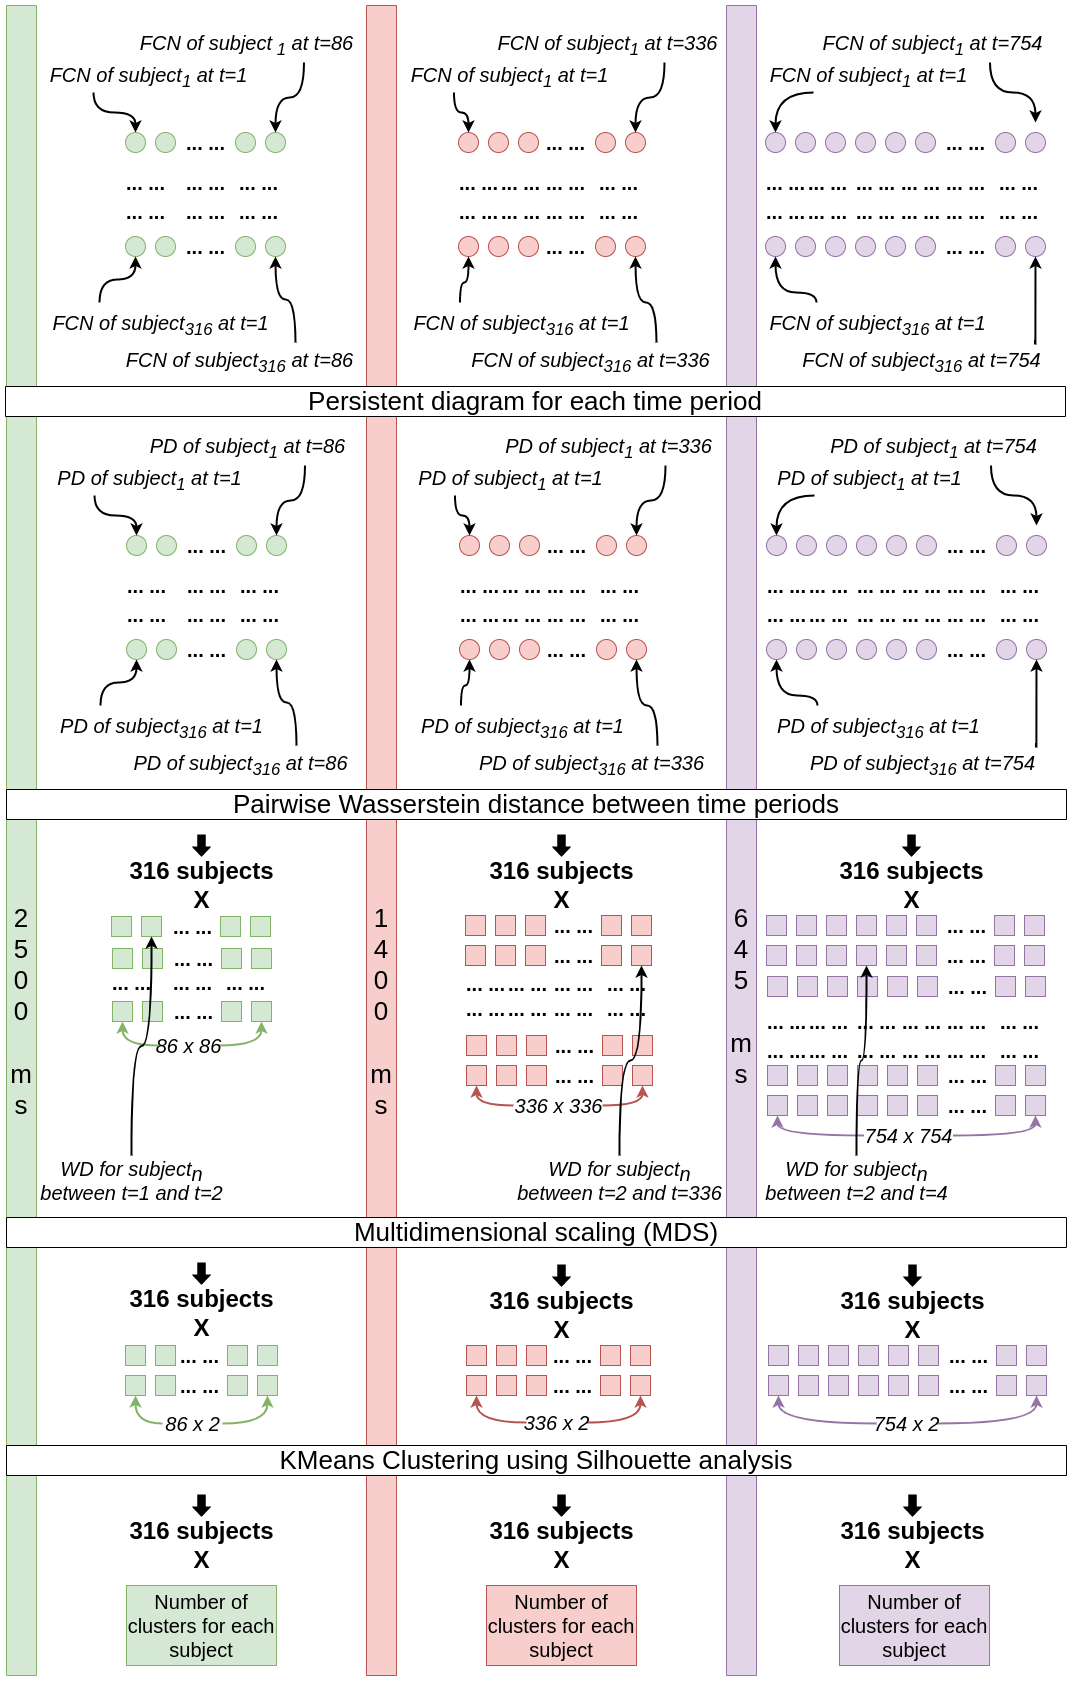
\includegraphics[height=0.9\textheight]{figures/tda_pipeline.png}
	\caption{TDA pipeline.}
	\label{fig:tda_pipeline}
\end{figure}

\subsection{Statistical analysis}
\label{sec:si}

A persistent barcode can be represented with a persistent diagram without information loss where the birth and death of a component (a topological feature) are represented as a point on the X-axis and Y-axis, respectively. These points on a two-dimensional surface as a \emph{persistent diagram} can be used for statistical inference to prove that persistent homology is resilient to different data acquisition parameters. The literature shows the usability of earth moving distance, also known as Wasserstein distance (WD), for statistical inference of persistent diagrams \cite{vallender1974calculation, edelsbrunner2013persistent}.

We use WD as a metric to compute the distance between two persistence diagrams extracted from two FCNs. WD represents the minimum value that is computed in the match calculation between the points of two persistent diagrams. The WD value of two similar persistent diagrams is smaller than two dissimilar persistent diagrams. This WD metric assists in proving the hypothesis of similarity between the persistent diagrams extracted from different data acquisition parameters, such as sampling rates. 

We develop two frameworks for statistical analysis: (a) topological data analysis framework and (b) traditional FCN analysis framework. We used Matlab during the data preprocessing steps and Python for statistical analysis. For the topological data analysis framework, we used \emph{Gudhi} library~\cite{jea_hera} to compute the 0-dimensional barcodes from FCNs and to calculate WD distances between the persistent diagrams. We also used \emph{scikit-learn} library for multidimensional scaling, and cluster calculation \cite{scikit-learn}.

\subsubsection{Topological data analysis framework}
\label{sec:tda_pipeline}




We develop a topological data analysis (TDA) framework to test our hypothesis of the similarity of the fMRI FCNs on different data acquisition parameters, such as different temporal sampling rates (TR). Our dataset includes three data cohorts: $645ms$, $1400ms$, and $2500ms$. For these TRs, each of the subjects (316 in total) has 754, 336, and 86 timesteps, respectively. Figure \ref{fig:tda_pipeline} represents the TDA pipeline we develop for the TDA framework. We calculate pairwise WD between the persistent diagrams of the timesteps for all subjects within the same data cohort. 

Let,
\begin{align*}
S_i & = \text{Subject } i, \text{ where } i = 1,2,\ldots,316 \\
T_k & = \text{Number of time steps for data cohort } k, 
\\
& \text{ where } k\in(645ms, 1400ms, 2500ms) \\
P_{S_i,t} & = \text{Persistence diagram for subject } S_i \text{ at time } t \\
d_W(P_1,P_2) & = \text{Wasserstein distance between persistence diagrams } P_1 \text{ and } P_2
\end{align*}

The TDA distance matrix for a given subject $S_i$ in cohort $k$ is defined as:
\begin{equation}
D(S_i)_{t_1,t_2} = d_W(P_{S_i,t_1}, P_{S_i,t_2}) \quad \text{for } t_1, t_2 = 1, \ldots, T_k \label{eq:tda_dis}
\end{equation}

In Eq. \ref{eq:tda_dis}, we compute the pairwise Wasserstein distance between persistence diagrams at times $t_1$ and $t_2$ which gives a $T_k \times T_k$ distance matrix for each subject $S_i$. We have three data cohorts ($645ms$, $1400ms$, $2500ms$) with different timesteps (754, 336, 86). Thus, we get 316 adjacency matrices for each data cohort with size ($754 \times 754$), ($336 \times 336$), and ($86 \times 86$), respectively.

\begin{figure}[!ht]%[!htb]
	\centering	
	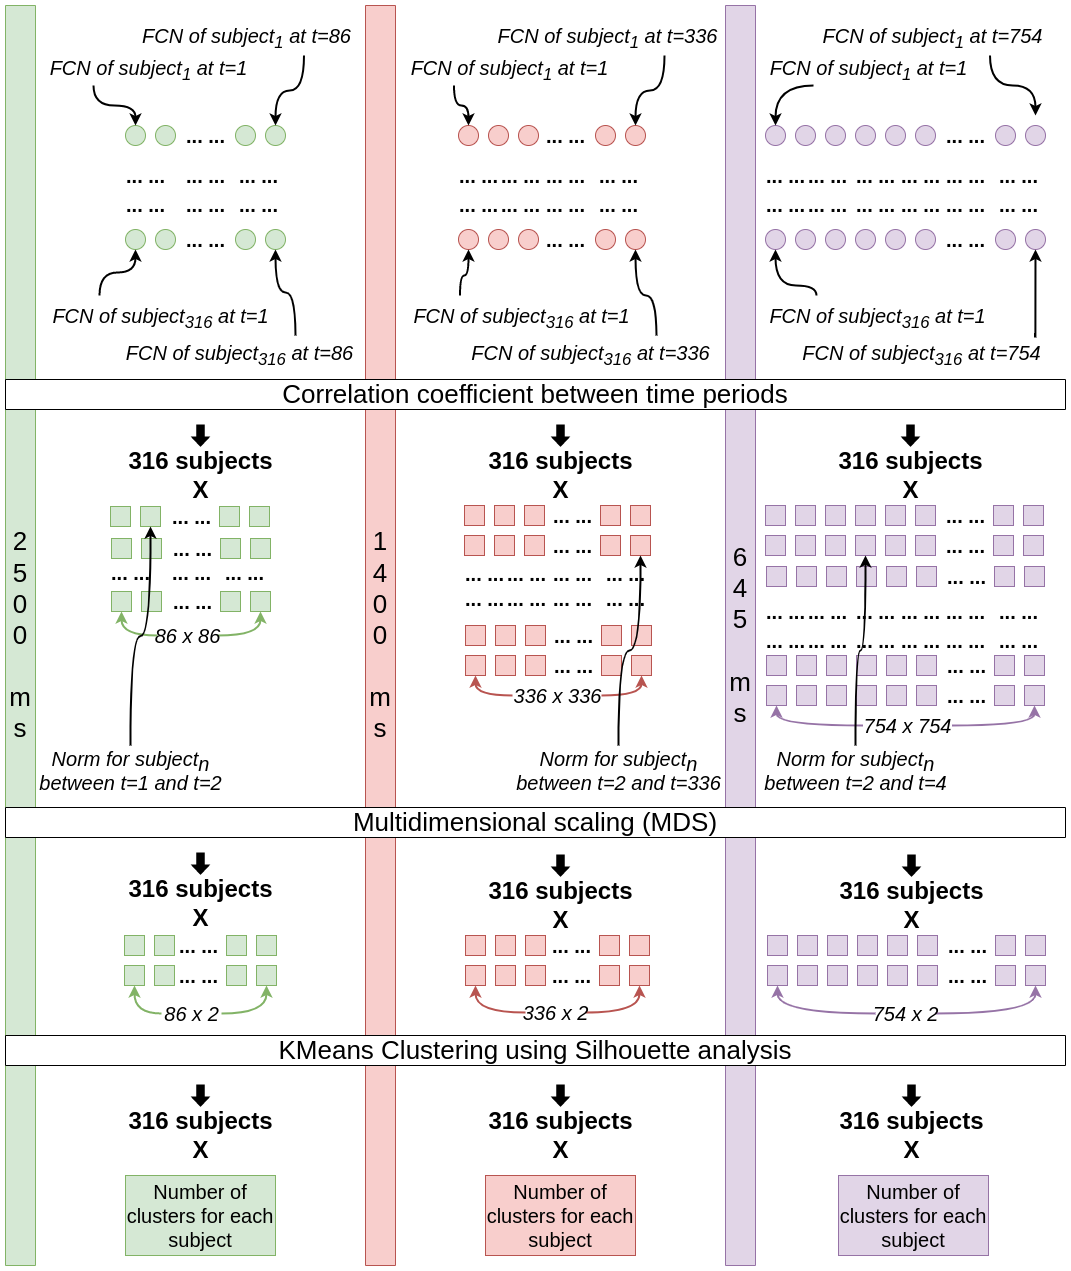
\includegraphics[height=0.9\textheight]{figures/non_tda_pipeline.png}
	\caption{Non TDA pipeline}
	\label{fig:nontda_pipeline}
\end{figure}

These high dimensional adjacency matrices are complex to analyze by statistical methods. To make it interpretable by the statistical methods, We apply two component multidimensional scaling (MDS) technique to reduce the dimensionality of the matrices. After this stage, we get 316 adjacency matrices for each data cohort with size ($ 754 \times 2 $), ($ 336 \times 2 $), and ($ 86 \times 2 $). The two-dimensional MDS results are plotted using scatter plots that give an intuition to use clustering to calculate the similarity between the TRs. We apply the k-means clustering technique to the MDS results to get the number of clusters for the reduced-sized matrices. As k-means clustering requires configuring the number of clusters $n$ before the cluster computation, we choose $n$ using a well-known approach called Silhouette analysis. Using Silhouette analysis, we choose $n$ that gives the maximum Silhouette score for the given adjacency matrices between the range from 2 to 16 \cite{scikit-learn, rousseeuw1987silhouettes}. After calculating the number of clusters for all three data cohorts, we get the number of clusters for all 316 subjects across these data cohorts. A similar number of clusters for the same subject across three data cohorts will indicate the similarity between the subjects for different data acquisition parameters (different TRs in our case). If we get significant similarity between the TRs, we can conclude the resiliency of persistent homology for rs-fMRI data analysis with different data acquisition parameters.



\subsubsection{Traditional FCN analysis}
\label{sec:nontda_pipeline}
Alongside the TDA framework, we also develop a nonTDA framework to show the efficiency of persistent homology over the traditional FCN analysis for the rs-fMRI dataset with different temporal sampling periods. The nonTDA framework is illustrated in Figure \ref{fig:nontda_pipeline}. Instead of the persistent diagrams or applying any persistent homology methods, we use a correlation coefficient between the timesteps for all three data cohorts. 


Let,
\begin{align*}
S_i &= \text{Subject } i, \text{ where } i = 1,2,\ldots,316 \\
T_k &= \text{Number of time steps for data cohort } k, \\
&\text{ where } k\in(645\text{ms}, 1400\text{ms}, 2500\text{ms}) \\
A_{S_i,t} &= \text{Adjacency matrix for subject } S_i \text{ at time } t
\end{align*}

The distance matrix for a given subject $S_i$ in cohort $k$ is defined as:

\begin{equation}
D(S_i)_{t_1,t_2} = \sqrt{\sum_{m=1}^{M} \sum_{n=1}^{N} |a_{mn}^{t_1} - a_{mn}^{t_2}|^2}
\label{eq:nontda_dis}
\end{equation}

In Eq. \ref{eq:nontda_dis}, $M, N$ are the dimensions of the adjacency matrices. We compute the Eucledean distance between adjacency matrices at times $t_1$ and $t_2$ which gives 316 distance matrices of sizes ($86 \times 86$), ($336 \times 336$), and ($754 \times 754$) for the three cohorts respectively. In this stage, we acquire 316 matrices for each of the data cohorts with the size of ($86 \times 86$) for $2500ms$,  ($336 \times 336$) for $1400ms$, and ($754 \times 754$) for $645ms$. Then we follow a similar pipeline of the TDA framework to keep the comparison uniform. We reduce the dimension of the matrices using two-component multidimensional scaling (MDS) and then calculate the number of clusters ($n$) on the reduced matrices using k-means clustering. We also use the maximum Silhouette score to choose the value of $n$ within the range from 2 to 16. Finally, this pipeline will also produce the number of clusters of the MDS for every 316 subjects for all three data cohorts. Our hypothesis will be proven right if the TDA pipeline gives a better similarity score than the nonTDA pipeline. 